\documentclass[10pt, a4paper,spanish]{article}

\usepackage[utf8]{inputenc}
\usepackage[spanish]{babel}

\usepackage[T1]{fontenc}

\usepackage[hmarginratio=1:1,top=32mm,columnsep=20pt]{geometry}
\usepackage[hang, small,labelfont=bf,up,textfont=it,up]{caption}

\usepackage{float}

\usepackage{amsmath}

\usepackage{enumitem}

\usepackage[hidelinks]{hyperref}

\usepackage{listings}
\usepackage{courier}


\lstset{
    language=bash,
    basicstyle=\ttfamily,
    keywordstyle=\bfseries,
    sensitive=false,
    morekeywords={, instanceOf, is, subClassOf, end, instance, daemon, ifNeeded, class, type, value, }
    showstringspaces=false,
    inputencoding=utf8,
    extendedchars=true,
		literate={á}{{\'a}}1 {é}{{\'e}}1 {í}{{\'i}}1 {ó}{{\'o}}1 {ú}{{\'u}}1 {ñ}{{\~n}}1,
}

\usepackage{graphicx}
\graphicspath{ {images/} }

\usepackage{titlesec}
\renewcommand\thesection{\Roman{section}}
\renewcommand\thesubsection{\Roman{subsection}}
\titleformat{\section}[block]{\large\scshape\centering}{\thesection.}{1em}{}
\titleformat{\subsection}[block]{\large}{\thesubsection.}{1em}{}

\usepackage{fancyhdr}
\pagestyle{fancy}
\fancyhead{}
\fancyfoot{}
\fancyhead[C]{ \today \ $\bullet$ Ingeniería del Conocimiento $\bullet$ Sistemas Basados en Marcos}
\fancyfoot[RO]{\thepage}

%-------------------------------------------------------------------------------
%	TITLE SECTION
%-------------------------------------------------------------------------------

\title{\vspace{-15mm}\fontsize{24pt}{10pt}\selectfont\textbf{Sistemas Basados en Marcos}} % Article title

\author{Sergio García Prado}
\date{\today}

%-------------------------------------------------------------------------------

\begin{document}

	\maketitle % Insert title

	\thispagestyle{fancy} % All pages have headers and footers

%-------------------------------------------------------------------------------
%	TEXT
%-------------------------------------------------------------------------------

  \section{Representar la siguiente descripción de los vasos sanguíneos mediante un sistema de marcos:}

		\begin{figure}[H]
			\begin{center}
				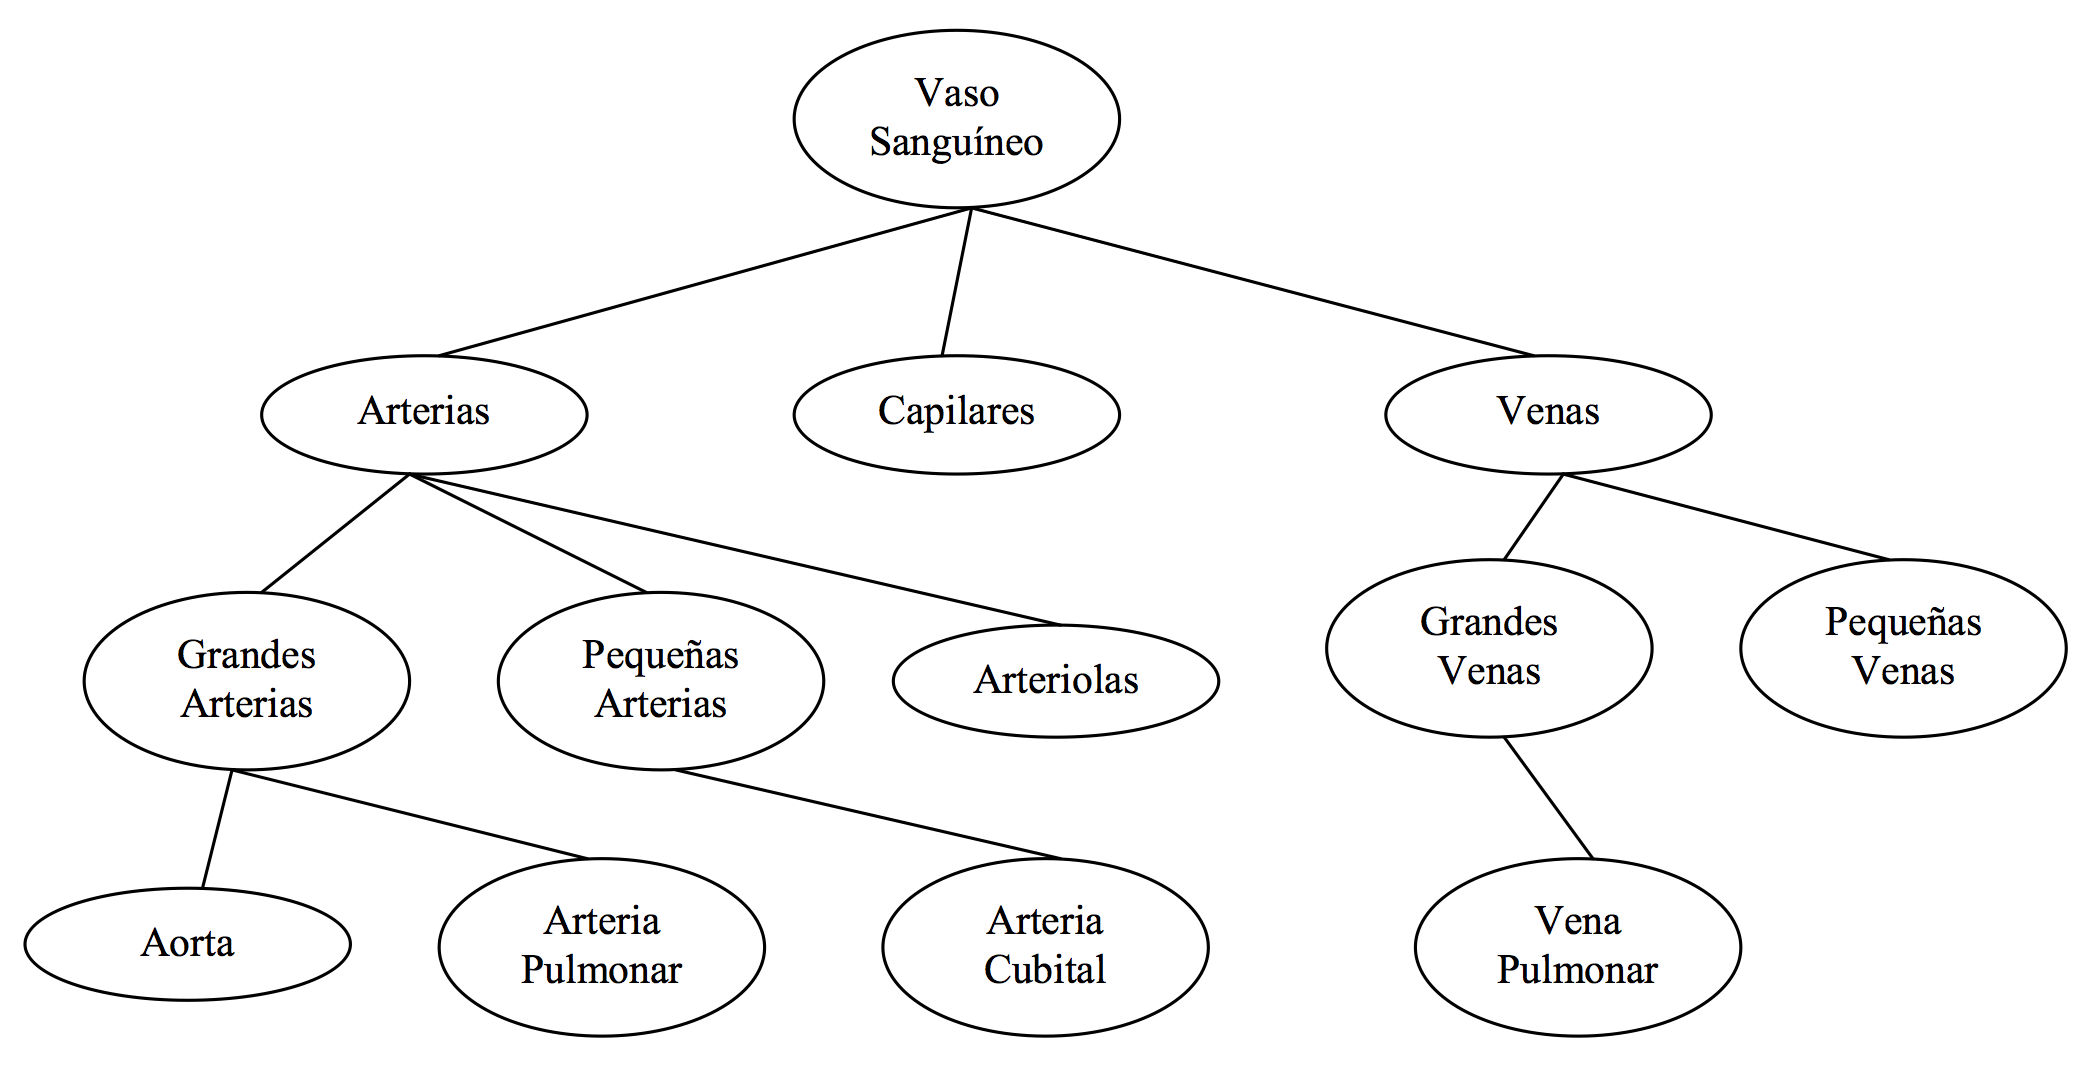
\includegraphics[width=0.75\textwidth]{diagram}
				\caption{Representación de los basos sanguíneos}
				\label{image:blood-vessel}
			\end{center}
		\end{figure}

    \begin{enumerate}[label=\alph*)]

      \item Los vasos sanguíneos tienen forma tubular y transportan sangre.

      \item Los vasos sanguíneos se subdividen en tres categorías: arterias, capilares y venas. Estas categorías se subdividen como indica la figura \ref{image:blood-vessel}.

      \item La aorta, la arteria y vena pulmonar y la arteria cubital son ejemplos de vasos sanguíneos específicos.

      \item Las arterias transportan sangre desde el corazón hasta los capilares de los tejidos y se distinguen de otros vasos por poseer una pared gruesa. En la mayoría de los casos, las arterias transportan sangre con un elevado contenido de oxígeno.

      \item Contrariamente a las arterias, las venas transportan sangre desde los capilares de los tejidos al corazón. Tienen una pared relativamente delgada. Usualmente, las venas contienen sangre pobre en oxígeno.

      \item La presión sanguínea media en las arterias es relativamente elevada (40-100 mmHg), frente a una presión media inferior a 10 mmHg en la mayoría de las venas.

      \item Las arterias pulmonares son un ejemplo de excepción a la descripción anterior. Estas arterias transfieren sangre del corazón a los pulmones y poseen una gruesa pared muscular. Por ello se las considera arterias. Sin embargo, estas arterias transfieren sangre con bajo contenido en oxígeno y su presión media es más bien baja (13 mmHg).

      \item Las grandes arterias tiene un diámetro entre 1 y 2,5 cm. Las pequeñas arterias tienen un diámetro de 0,4 cm. y las arteriolas de 0,003 cm.

      \item Las grandes venas tienen un diámetro entre 3 y 1,5 cm. y las pequeñas venas tienen un diámetro de 0,5 cm.

      \item La arteria aorta tiene un diámetro de 2,5 cm.

      \item La arteria pulmonar izquierda tiene un diámetro de 1,4 cm.

      \item La vena cava tiene un diámetro de 3 cm.

    \end{enumerate}

		\paragraph{}

		\subsection{Clases}

			\begin{figure}[H]
				\centering
        \lstinputlisting{pseudocode/exercise1/vasoSanguineo.frame}
			\end{figure}

			\begin{figure}[H]
				\centering
        \lstinputlisting{pseudocode/exercise1/arteria.frame}
			\end{figure}

			\begin{figure}[H]
				\centering
        \lstinputlisting{pseudocode/exercise1/vena.frame}
			\end{figure}

			\begin{figure}[H]
				\centering
        \lstinputlisting{pseudocode/exercise1/capilar.frame}
			\end{figure}

			\begin{figure}[H]
				\centering
        \lstinputlisting{pseudocode/exercise1/granArteria.frame}
			\end{figure}

			\begin{figure}[H]
				\centering
        \lstinputlisting{pseudocode/exercise1/pequenaArteria.frame}
			\end{figure}

			\begin{figure}[H]
				\centering
        \lstinputlisting{pseudocode/exercise1/arteriola.frame}
			\end{figure}

			\begin{figure}[H]
				\centering
        \lstinputlisting{pseudocode/exercise1/granVena.frame}
			\end{figure}

			\begin{figure}[H]
				\centering
        \lstinputlisting{pseudocode/exercise1/pequenaVena.frame}
			\end{figure}

		\subsection{Instancias}

			\begin{figure}[H]
				\centering
        \lstinputlisting{pseudocode/exercise1/aorta.frame}
			\end{figure}

			\begin{figure}[H]
				\centering
        \lstinputlisting{pseudocode/exercise1/arteriaPulmonarIzquierda.frame}
			\end{figure}

			\begin{figure}[H]
				\centering
        \lstinputlisting{pseudocode/exercise1/arteriaCubital.frame}
			\end{figure}

			\begin{figure}[H]
				\centering
        \lstinputlisting{pseudocode/exercise1/venaPulmonar.frame}
			\end{figure}

			\begin{figure}[H]
				\centering
        \lstinputlisting{pseudocode/exercise1/venaCaba.frame}
			\end{figure}

		\subsection{Diagrama}

			\begin{figure}[H]
				\begin{center}
					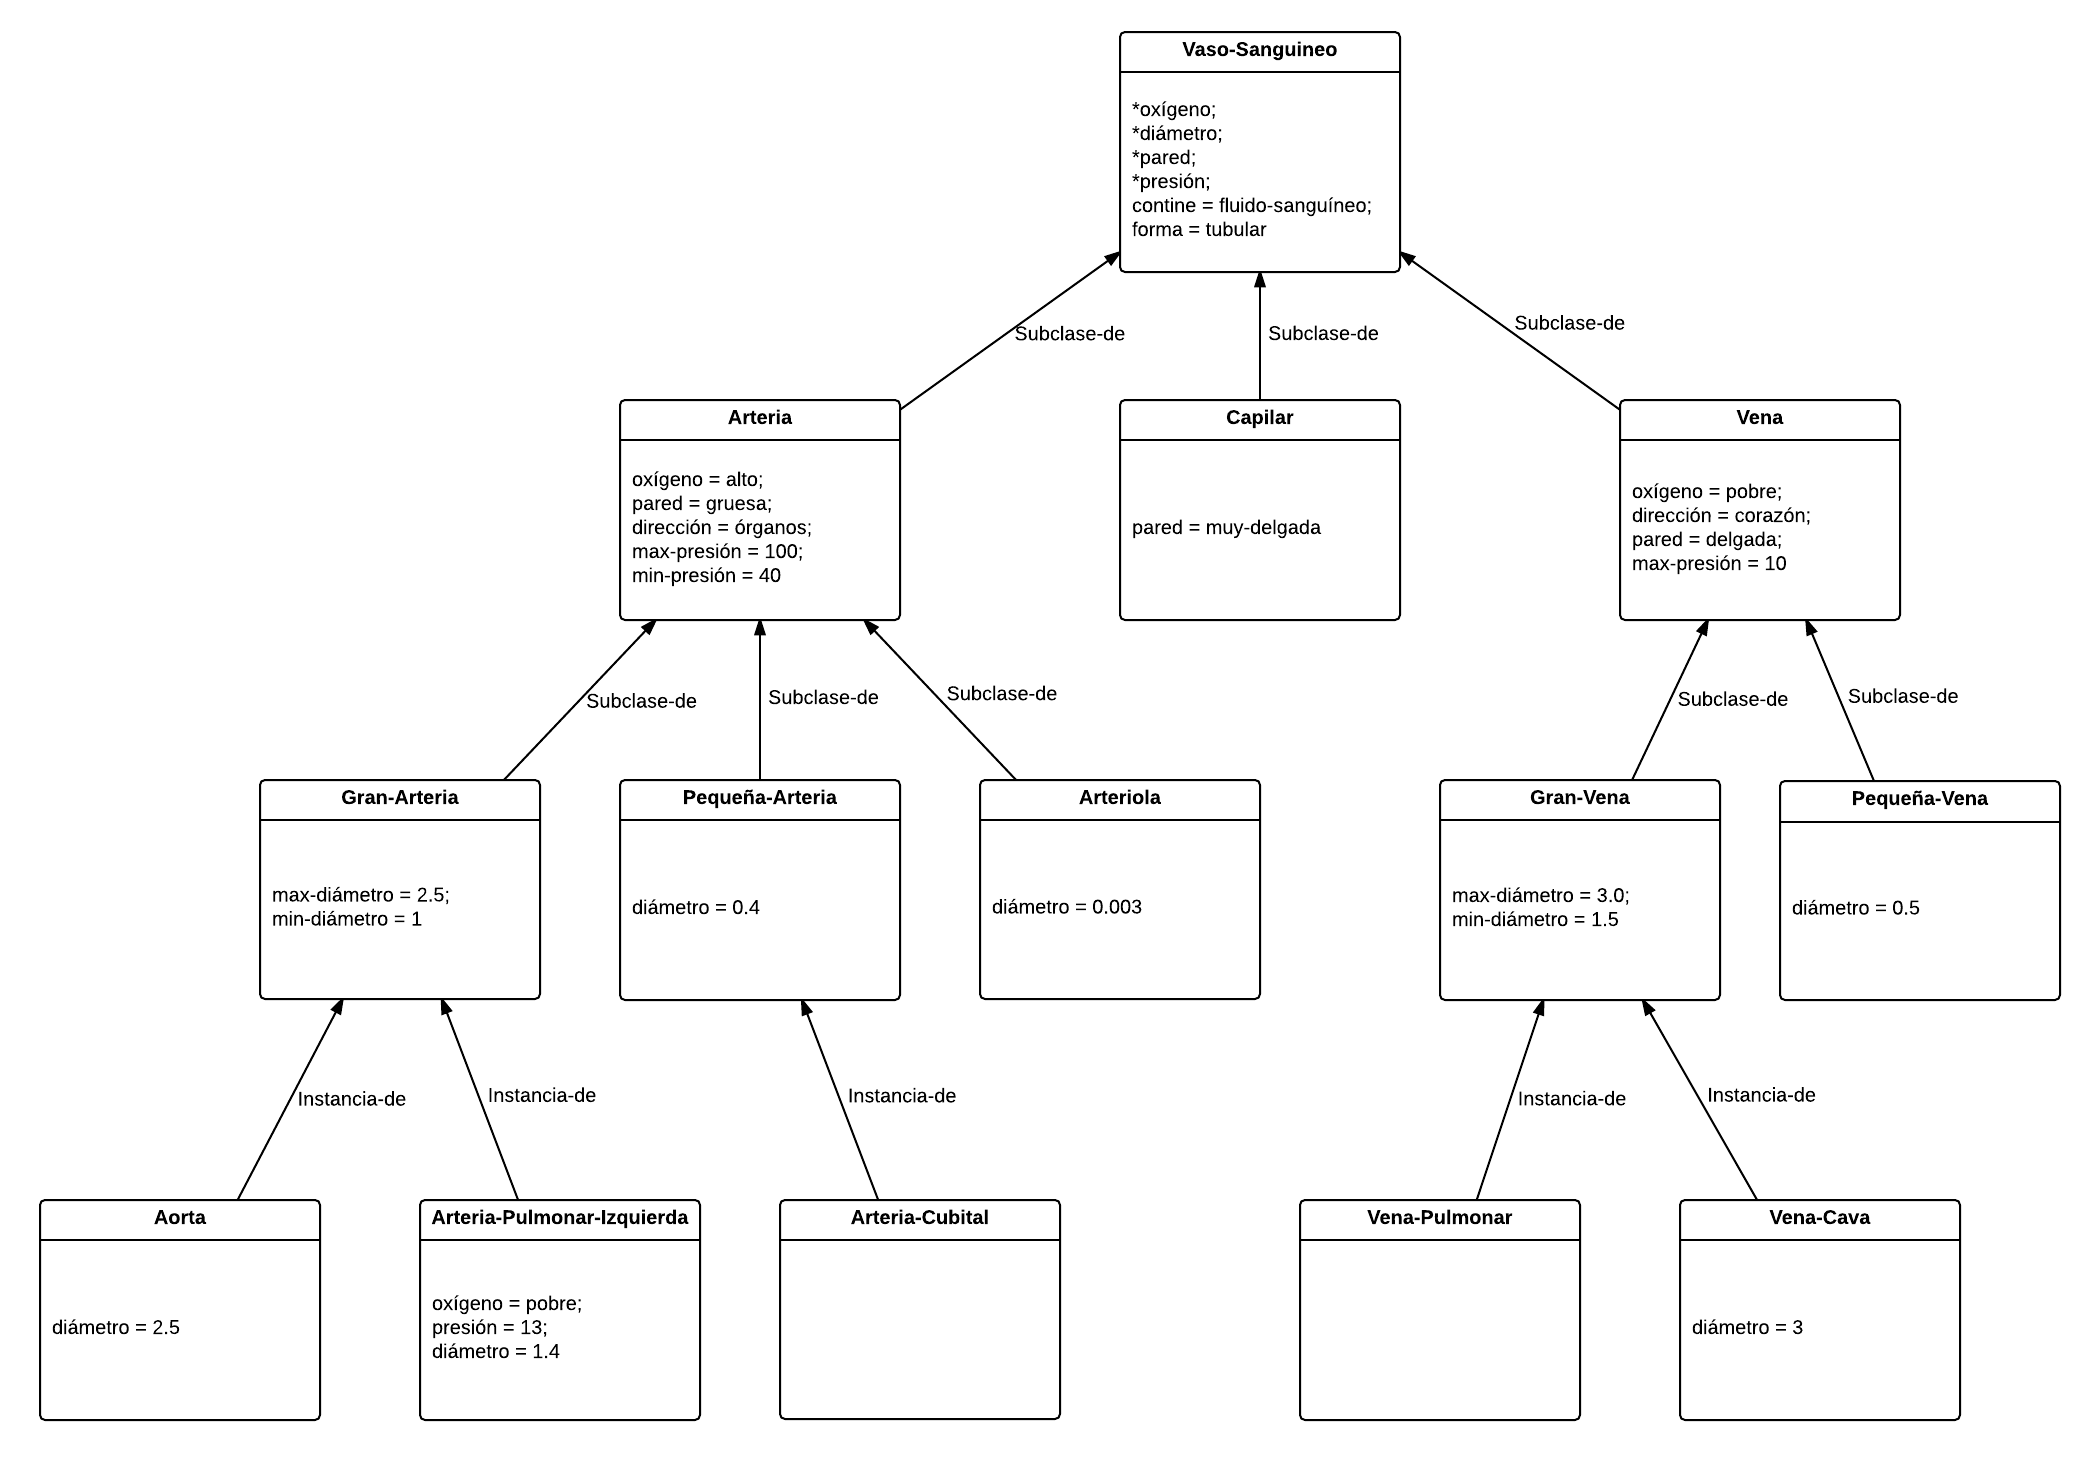
\includegraphics[width=\textwidth]{exercise-1-diagram}
					\caption{Ejercicio 1: Diagrama de Clases e Instancias}
					\label{image:diagram-1}
				\end{center}
			\end{figure}


	\section{Elaborar una jerarquía de marcos con herencia múltiple. La jerarquía debe de permitir obtener el área y el perímetro de cualquier polígono regular, así como el área de cualquier cuadrilátero. También debe permitir obtener la base, altura y apotema de cualquier cuadrado:}

		\begin{enumerate}[label=\alph*)]

			\item Un polígono es una figura geométrica cerrada y plana limitada por tres o más líneas rectas que se cortan en sus vértices.

			\item Un polígono regular es aquel cuyos ángulos $\alpha$ son iguales, y cuyos lados $l$ tienen la misma longitud. El segmento que une el centro del polígono con el punto medio de cualquiera de sus lados es la apotema.

			\item El perímetro de un polígono regular es el producto de su número de lados por la longitud del lado.

			\item Al área de un polígono regular es la mitad del producto de su perímetro por su apotema

			\item Un cuadrilátero es un polígono de cuatro lados.

			\item El área de un cuadrilátero es el producto de su base por la altura.

			\item Los cuadrados tienen los lados y los ángulos iguales. Su apotema mide la mitad del lado.

		\end{enumerate}

    \subsection{Clases}

			\begin{figure}[H]
				\centering
        \lstinputlisting{pseudocode/exercise2/poligono.frame}
			\end{figure}

			\begin{figure}[H]
				\centering
        \lstinputlisting{pseudocode/exercise2/poligonoRegular.frame}
			\end{figure}

			\begin{figure}[H]
				\centering
        \lstinputlisting{pseudocode/exercise2/cuadrilatero.frame}
			\end{figure}

			\begin{figure}[H]
				\centering
        \lstinputlisting{pseudocode/exercise2/cuadrado.frame}
			\end{figure}

    \subsection{Diagrama}

			\begin{figure}[H]
				\begin{center}
					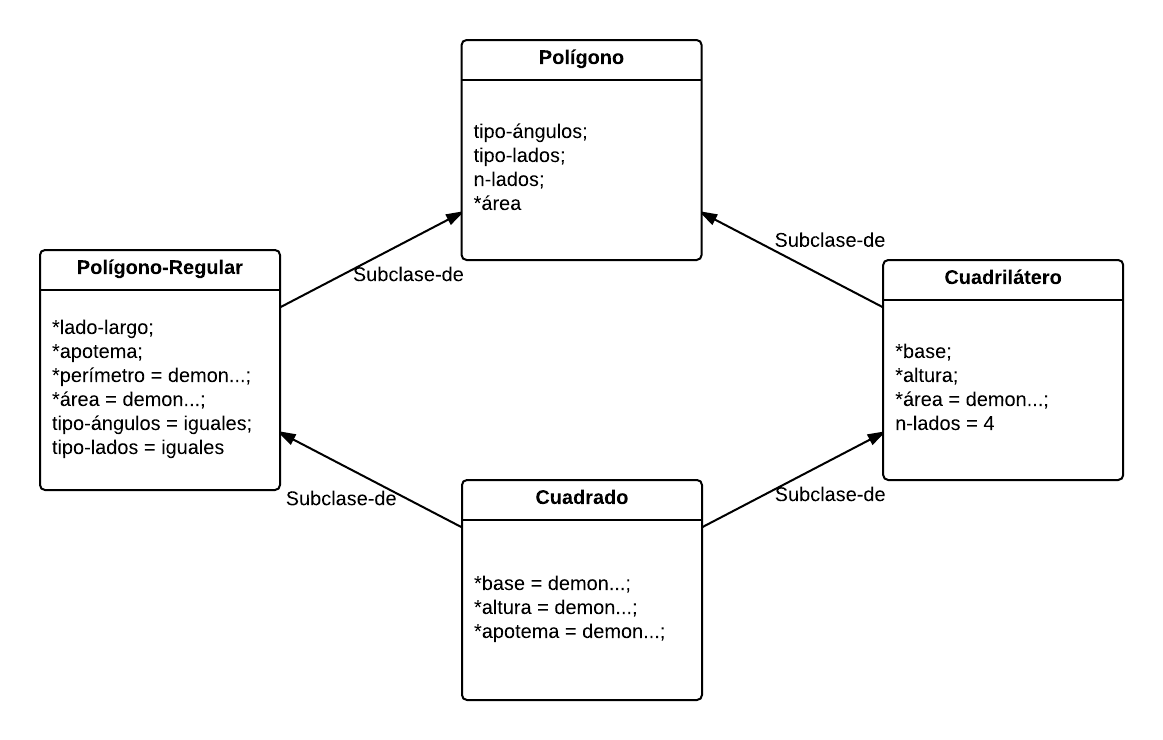
\includegraphics[width=\textwidth]{exercise-2-diagram}
					\caption{Ejercicio 2: Diagrama de Clases}
					\label{image:diagram-2}
				\end{center}
			\end{figure}

    \subsection{Contradicciones}

      \paragraph{}
      Existe una contradicción debido a la herencia múltiple del modelo de marcos diseñado. Esta sucede en la propiedad \textbf{área} de la clase \textbf{cuadrado}, que tiene dos implementaciones al mismo nivel de herencia. Estas se corresponden con los demonios \emph{AreaPolRegular} y \emph{AreaCuadrilatero}

\end{document}
